% HB9ARK 22-SEP-2026
% Mechanisches Analogon einer Diode, das der Veranschaulichung dienen kann. 
% In der einen Richtung fliesst nie Wasser.
% In der anderen Richtung kann Wasser nach der Überwindung eines Schwellwerts fliessen.
\documentclass[tikz,border=4mm]{standalone}
\usepackage{tikz}
\usepackage{amsmath}
\usetikzlibrary{arrows.meta,decorations.pathreplacing}
\begin{document}
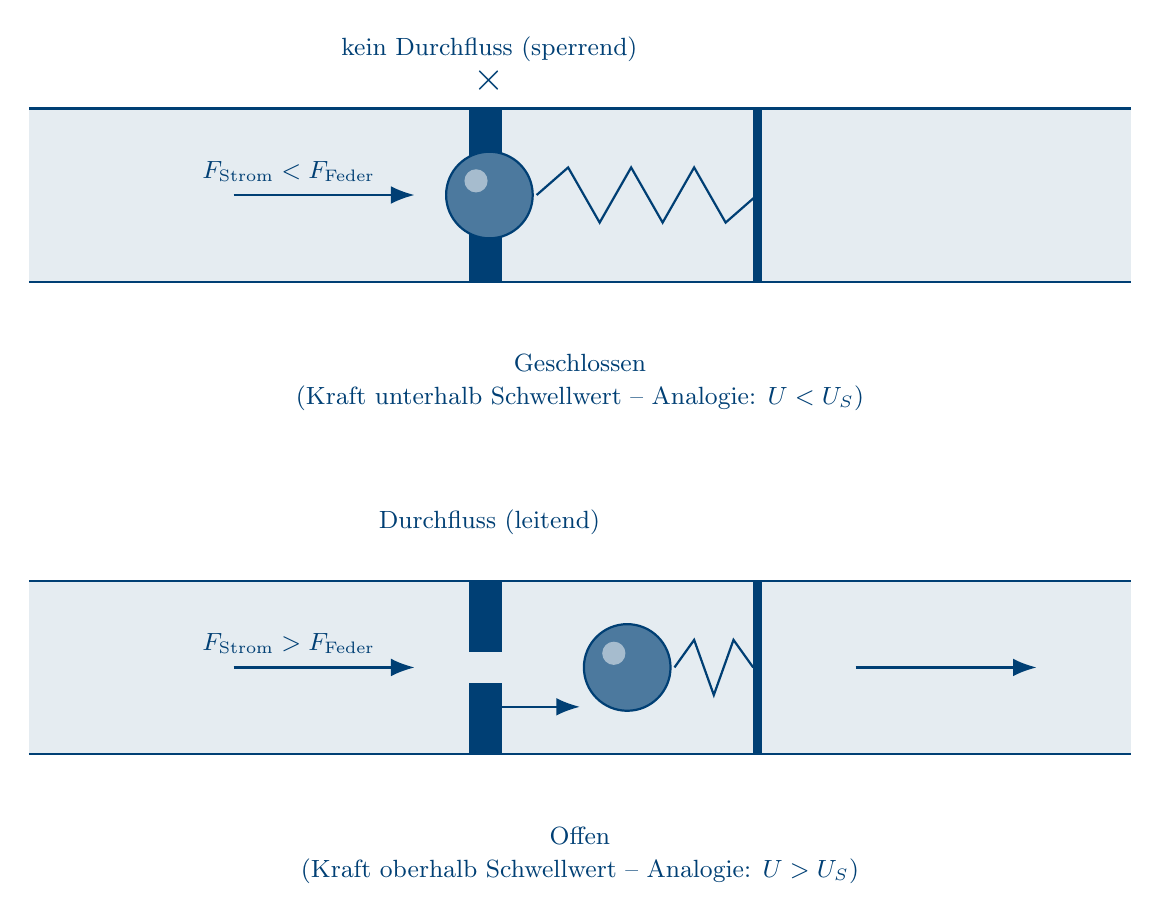
\begin{tikzpicture}[scale=1]
\definecolor{DARCblue}{RGB}{0,63,116}

% ======================= PANEL 1 (oben): GESCHLOSSEN / SPERREND =======================
\begin{scope}[yshift=6cm]
  \fill[DARCblue!10] (0,0.4) rectangle (14,2.6);
  \draw[DARCblue, thick] (0,0.4) -- (14,0.4);
  \draw[DARCblue, thick] (0,2.6) -- (14,2.6);

  % Ventilsitz
  \filldraw[DARCblue, draw=DARCblue] (5.6,0.4) rectangle (6.0,1.3);
  \filldraw[DARCblue, draw=DARCblue] (5.6,1.7) rectangle (6.0,2.6);

  % Kugel: geschlossen auf dem Sitz
  \filldraw[DARCblue!70, draw=DARCblue, thick] (5.85,1.5) circle (0.55);
  \filldraw[DARCblue!35] (5.68,1.68) circle (0.14);

  % Feder: entspannt (volle Laenge)
  \draw[DARCblue, thick]
    (6.45,1.5) -- (6.85,1.85) -- (7.25,1.15) -- (7.65,1.85) -- (8.05,1.15) -- (8.45,1.85) -- (8.85,1.15) -- (9.25,1.5);
  \filldraw[DARCblue] (9.2,0.4) rectangle (9.3,2.6);

  % Kraftpfeile
  \draw[-{Latex[length=3mm]}, DARCblue, thick] (2.6,1.5) -- (4.9,1.5);
  \node[above, DARCblue] at (3.3,1.55) {\small $F_{\text{Strom}} < F_{\text{Feder}}$};
  \node[DARCblue, thick] at (5.85,2.95) {\Large $\times$};
  \node[DARCblue] at (5.85,3.35) {\small kein Durchfluss (sperrend)};

  \node[below, DARCblue, align=center] at (7,-0.4)
    {\small Geschlossen \\ \small (Kraft unterhalb Schwellwert -- Analogie: $U<U_S$)};
\end{scope}

% ======================= PANEL 2 (unten): OFFEN / LEITEND =======================
\begin{scope}
  \fill[DARCblue!10] (0,0.4) rectangle (14,2.6);
  \draw[DARCblue, thick] (0,0.4) -- (14,0.4);
  \draw[DARCblue, thick] (0,2.6) -- (14,2.6);

  % Ventilsitz
  \filldraw[DARCblue, draw=DARCblue] (5.6,0.4) rectangle (6.0,1.3);
  \filldraw[DARCblue, draw=DARCblue] (5.6,1.7) rectangle (6.0,2.6);

  % Kugel: abgehoben, gibt die Bohrung frei
  \filldraw[DARCblue!70, draw=DARCblue, thick] (7.6,1.5) circle (0.55);
  \filldraw[DARCblue!35] (7.43,1.68) circle (0.14);

  % Feder: komprimiert (kuerzer)
  \draw[DARCblue, thick]
    (8.2,1.5) -- (8.45,1.85) -- (8.7,1.15) -- (8.95,1.85) -- (9.2,1.5);
  \filldraw[DARCblue] (9.2,0.4) rectangle (9.3,2.6);

  % Durchfluss: Pfeile durch die geoeffnete Bohrung hindurch
  \draw[-{Latex[length=3mm]}, DARCblue, thick] (2.6,1.5) -- (4.9,1.5);
  \node[above, DARCblue] at (3.3,1.55) {\small $F_{\text{Strom}} > F_{\text{Feder}}$};
  \draw[-{Latex[length=3mm]}, DARCblue, thick] (5.8,1.0) -- (7.0,1.0);
  \draw[-{Latex[length=3mm]}, DARCblue, thick] (10.5,1.5) -- (12.8,1.5);
  \node[DARCblue] at (5.85,3.35) {\small Durchfluss (leitend)};

  \node[below, DARCblue, align=center] at (7,-0.4)
    {\small Offen \\ \small (Kraft oberhalb Schwellwert -- Analogie: $U>U_S$)};
\end{scope}

\end{tikzpicture}
\end{document}
